% This is file JFM2esam.tex
% first release v1.0, 20th October 1996
%       release v1.01, 29th October 1996
%       release v1.1, 25th June 1997
%       release v2.0, 27th July 2004
%       release v3.0, 16th July 2014
%       release v4.0, 15th June 2017
%   (based on JFMsampl.tex v1.3 for LaTeX2.09)
% Copyright (C) 1996, 1997, 2014, 2017 Cambridge University Press

\documentclass[12pt, a4paper]{article}
\usepackage{graphicx}
% \usepackage{epstopdf, epsfig}

\usepackage{graphicx}
\usepackage{times}
\usepackage{tabularx}
\usepackage{fancyhdr}
\usepackage{pbox}
\usepackage[utf8]{inputenc}
\usepackage[T1]{fontenc}
\usepackage{amsmath}
\usepackage{setspace}
\usepackage[a4paper, left=25mm, right=25mm, top=30mm, bottom=30mm]{geometry}
\usepackage{titlesec}

% \usepackage[square, comma, sort&compress, numbers]{natbib}
% \bibliographystyle{IEEEtran}
% \usepackage{cite}
\usepackage[style=ieee]{biblatex}



\newcommand{\wideunderline}[2][2em]{%
  \underline{\parbox[t]{#1}{\centering{#2}}}%
}

% \renewcommand\footnotesize{\small}
% \newcommand\indexsize{\@setfontsize\indexsize\@viiipt\@ixpt}
% \renewcommand\scriptsize{\@setfontsize\scriptsize\@viipt\@viiipt}
% \renewcommand\tiny{\@setfontsize\tiny\@vpt\@vipt}
% \renewcommand\large{\@setfontsize\large\@xipt{13}}
% \renewcommand\Large{\@setfontsize\Large\@xivpt{18}}
% \renewcommand\LARGE{\@setfontsize\LARGE\@xviipt{19}}
% \renewcommand\huge{\@setfontsize\huge\@xxpt{25}}
% \renewcommand\Huge{\@setfontsize\Huge\@xxvpt{30}}

\newcommand\SectionSize{\@setfontsize\SectionSize{15}{22.5}}
\newcommand\ArticleSize{\@setfontsize\ArticleSize{14}{21}}
\newcommand\ItemSize{\@setfontsize\ItemSize{12}{18}}

\titleformat{\section}
  {\normalfont\fontsize{15}{22.5}\bfseries}{\thesection}{1em}{}
\titleformat{\subsection}
  {\normalfont\fontsize{14}{21}\bfseries}{\thesubsection}{1em}{}
\titleformat{\subsubsection}
  {\normalfont\fontsize{12}{18}\bfseries}{\thesubsubsection}{1em}{}

% \def\@maketitle{%
%   \newpage
%   \null
%   \vskip 2em%
%   \begin{center}%
%     \LARGE \@title \par
%   \end{center}%
%   \par
%   \vskip 1.5em}


% \redef\@maketitle#1{%
%  \newpage
%  \vspace*{10\p@}%
%  {\centering \sloppy
%   {\normalfont\LARGE\fontswitch\bfseries
%   \put@rapidsHead%
%   \@title@alignment%
%   \@title \par}%
%   \vskip 8\p@ \@plus 2\p@ \@minus 1\p@
%   {\normalfont\large\fontswitch\bfseries\baselineskip=12\p@
%      \@author@alignment%
%      \lowercase{\@author}\par}%
%   \vskip 4\p@ \@plus 1\p@
%   {\normalfont\small
%   \@aff@alignment%
%   \@affiliation \par}%
%   \vskip 8\p@ \@plus 2\p@ \@minus 1\p@
%   %{\normalfont\small (Received \@date)}% x@rem
%   \normalfont\small
%   \@history@alignment%
%   % (Received xx; revised xx; accepted xx)\hfill% x@add
%   \put@absrule
%  \par}%
%  \vskip 8\p@ \@plus 2\p@ \@minus 1\p@
% }

% \renewenvironment{abstract}
%   {\par\normalfont\normalsize\noindent\ignorespaces}
%   {\par\vskip 9\p@ \@plus 1\p@ \@minus 1\p@
% %   \vbox{\centerline{\rule[4\p@]{30pc}{.4\p@}}}
% }



\bibliography{reference/reference.bib}

\newtheorem{lemma}{Lemma}
\newtheorem{corollary}{Corollary}


\title{Title of RBM Research Proposal}


\begin{document}

\newcommand{\GroupProjectTitle}{Your Group Project Title, Some people always make it very long long long long long and now it can fit this situation}
\newcommand{\SubProjectTitle}{Your Sub Project Title}

\newcommand{\StudentName}{First Name . Last Name}
\newcommand{\StudentID}{5000XXXX}
\newcommand{\Email}{your.id@connect.hkust-gz.edu.cn}
\newcommand{\Supervisor}{Lionel M. NI}
\newcommand{\HubThrust}{Info Hub / DSA Thrust}
\newcommand{\ProjectMentor}{Ke XUE}



\begin{titlepage}
    \begin{center}
        \vspace*{1cm}

        \huge
        \textbf{HKUST (GZ)}
        \vspace{0.5cm}

        \textbf{Master Thesis Proposal for MPhil Degree}

        \vspace{3cm}
        
        \begin{minipage}{0.8\textwidth}
            \Large
            \centering

            \begin{tabular}{l@{}ll}
                \textbf{Student Name}\vspace{0.5cm} &     & \wideunderline[18em]{\StudentName} \\
                \textbf{ID Number}\vspace{0.5cm} &     & \wideunderline[18em]{\StudentID} \\
                \textbf{Email}\vspace{1.5cm} &     & \wideunderline[18em]{\Email} \\
                \textbf{Group Project}\vspace{0.5cm} &     & \wideunderline[18em]{{\GroupProjectTitle}} \\ 
                \textbf{Project Mentor}\vspace{1.5cm} &     & \wideunderline[18em]{\ProjectMentor} \\
                \textbf{Individual Project}\vspace{0.5cm}&     & \wideunderline[18em]{{\IndividualProjectTitle}}  \\
                \textbf{Prime Supervisor}\vspace{0.2cm} &     & \wideunderline[18em]{{\PrimeSupervisor}}  \\
                \textbf{Hub/Thrust}\vspace{0.5cm} &     & \wideunderline[18em]{\HubThrustPrime} \\
                \textbf{Co-supervisor}\vspace{0.2cm} &     & \wideunderline[18em]{\CoSupervisor} \\
                \textbf{Hub/Thrust} &     & \wideunderline[18em]{\HubThrustCo} \\
            \end{tabular}

        \end{minipage}

        
        
        \vfill
        
        \LARGE
        \textbf{Division of RBM} 
             
    \end{center}
 \end{titlepage}

\spacing{1.5}

\pagenumbering{roman}
\setcounter{page}{2}
\tableofcontents
\newpage

\setcounter{page}{1}
\pagenumbering{arabic}

\section{Introduction to the Group Project}

\subsection{Background and Objective}

Briefly describe the group project.


\subsection{Significance}

Explain why this group project is essential in the real-world context.


\subsection{Project Composition}

Provide information of the individual projects that collectively comprise the group
project, including titles/researcher names of each individual project.

\subsection{Project Connections}

Outline the connections between the group project and the individual projects.


\subsection{Project Milestones}

List the key milestones at different stages of the group project implementation.


\section{Proposal of the Individual Project}

\subsection{Significance and Relevance of the Individual Project to the Group Project}

\subsubsection{Complementary Role}

Explain how your project complements the broader objectives of the group project.
Discuss how your work fills a necessary gap or adds a unique perspective to the
collective effort.

\subsubsection{Value Addition}

Describe the specific ways in which your project adds value to the group project.
This might include the development of critical components, providing specialized
knowledge or skills, or enhancing the overall quality and scope of the group
project.

\subsubsection{Interdependence}


Highlight any dependencies between your project and other components of the
group project. Explain how collaboration and coordination with other group
members are integral to achieving both individual and group objectives.


\subsection{Statement of the Individual Project in Details}


\subsubsection{Literature/Market Review and Problem Definition}

\subsubsection{Objective and Scope of the Project}

\subsubsection{Research Method and Justification}

\subsubsection{Execution Plan}

\subsubsection{Intended Outcomes}

Outcome 1: Description \& relation of this outcome to the group project. \\
Outcome 2: Description \& relation of this outcome to the group project. \\
Outcome 3: Description \& relation of this outcome to the group project. \\

\subsection{Project Milestones}

Table the group project and the individual project milestones. Illustrate the relation
and alignment of milestones of the individual project and those of the group project.

\subsection{Budget Plan}

\subsubsection{Estimated Budget}

\subsubsection{Budget Breakdown}

Break down the budget into categories.

\subsubsection{Cost-Effectiveness}

Discuss cost-effectiveness.

\subsection{Risk Analysis and Mitigation}

\subsubsection{Potential Risks or Challenges}

Identify potential risks or challenges that may arise during implementation of the
project.

\subsubsection{Impact of the Risks}

Assess the impact of the risks to the success of the project and propose
mitigation strategies.

\section{Figures}
Figures should be as small as possible while displaying clearly all the information required, and with all lettering readable. Every effort should be taken to avoid figures that run over more than one page. There is no charge for colour figures. For review purposes figures should be embedded within the manuscript. Upon final acceptance, however, individual figure files will be required for production. These should be submitted in EPS or high-resolution TIFF format (1200 dpi for lines, 300 dpi for halftone, and 600 dpi for a mixture of lines and halftone). The minimum acceptable width of any line is 0.5pt. Each figure should be accompanied by a single caption, to appear beneath, and must be cited in the text. Figures should appear in the order in which they are first mentioned in the text and figure files must be named accordingly to assist the production process (and numbering of figures should continue through any appendices). For example see figures \ref{fig:ka} and \ref{fig:kd}. Failure to follow figure guidelines may result in a request for resupply and a subsequent delay in the production process.

\begin{figure}[htbp]
  \centering
  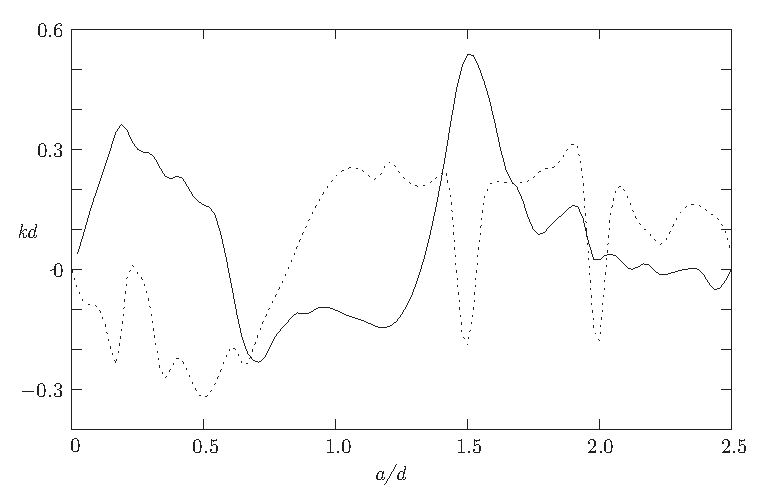
\includegraphics{image/trapped.eps}% Images in 100% size
  \caption{Trapped-mode wavenumbers, $kd$, plotted against $a/d$ for
    three ellipses:\protect\\%
    ---$\!$---,
    $b/a=1$; $\cdots$\,$\cdots$, $b/a=1.5$.}
\label{fig:ka}
\end{figure}

\begin{figure}
  \centering
  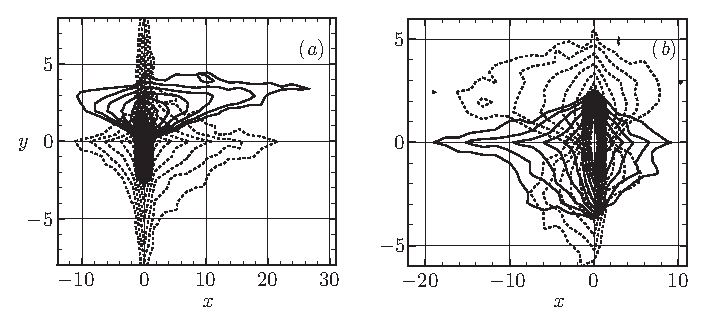
\includegraphics{image/modes}
  \caption{The features of the four possible modes corresponding to
  (\textit{a}) periodic\protect\\ and (\textit{b}) half-periodic solutions.}
\label{fig:kd}
\end{figure}

\subsection{Tables}
Tables, however small, must be numbered sequentially in the order in which they are mentioned in the text. The word \textit {table} is only capitalized at the start of a sentence. See table \ref{tab:kd} for an example.

\begin{table}
  
  \begin{center}
\def~{\hphantom{0}}
  \begin{tabular}{lccc}
      $a/d$  & $M=4$   &   $M=8$ & Callan \\[3pt]
       0.1   & 1.56905 & ~~1.56~ & 1.56904\\
       0.3   & 1.50484 & ~~1.504 & 1.50484\\
       0.55  & 1.39128 & ~~1.391 & 1.39131\\
       0.7   & 1.32281 & ~10.322 & 1.32288\\
       0.913 & 1.34479 & 100.351 & 1.35185\\
  \end{tabular}
  \caption{Values of $kd$ at which trapped modes occur when $\rho(\theta)=a$}
  \label{tab:kd}
  \end{center}
\end{table}

\section{Citations and references}

%All papers included in the References section must be cited in the article, and vice versa. Citations should be included as, for example ``It has been shown \citep{Rogallo81} that...'' (using the {\verb}\citep} command, part of the natbib package) ``recent work by \citet{Dennis85}...'' (using {\verb}\citet}).
The natbib package can be used to generate citation variations, as shown below. \cite{ngFederatedBayesianNetwork2022}

% \begin{itemize}
% \item \verb#\citet[pp. 2-4]{Galtier00}#:
% \citet[pp. 479-480]{Galtier00} 
% \item \verb#\citep[p. 6]{Worster92}#:
% \citep[p. 6]{Worster92}
% \item \verb#\citep[see][]{Koch83, Lee71, Linton92}#:
% \citep[see][]{Koch83, Lee71, Linton92}
% \item \verb#\citep[see][p. 18]{Martin80}#:
% \citep[see][p. 18]{Martin80}
% \item \verb#\citep{Brownell04,Brownell07,Ursell50,Wijngaarden68,Miller91}#:
% \citep{Brownell04,Brownell07,Ursell50,Wijngaarden68,Miller91}
% \end{itemize}

The References section can either be built from individual \verb#\bibitem# commands, or can be built using BibTex. The BibTex files used to generate the references in this document can be found in the zip file in the Instructions for Contributors section of the JPP website.

Where there are up to ten authors, all authors' names should be given in the reference list. Where there are more than ten authors, only the first name should appear, followed by et al.

Acknowledgements should be included at the end of the paper, before the References section or any appendicies, and should be a separate paragraph without a heading. Several anonymous individuals are thanked for contributions to these instructions.

\appendix

\section{}\label{appA}
This appendix contains sample equations in the JPP style. Please refer to the {\LaTeX} source file for examples of how to display such equations in your manuscript.



% susie put cite commands here, don't bother with citet etc just yet.

% \bibliographystyle{jpp}
% Note the spaces between the initials



% \bibliography{jpp-instructions}
\printbibliography
% \bibliography{reference/reference2}


\end{document}
